% !TeX root = probability.tex

%%%%%%%%%%%%%%%%%%%%%%%%%%%%%%%%%%%%%%%%%%%%%%%%%%%%%%%%

\section*{המלצות}

\addcontentsline{toc}{section}{\large המלצות}


קיץ תשפ"ב מועד ב. שים לב ש "מבין" ו "ידוע" לא מכוונים להסתברות מותנית. קיץ תשפ"א מועד א.

קיץ תשפ"ב מועד א. אני שמח לראות שבשאלה זו כותבים במפורש שתוצאות המשחקים בסדרה הן בלתי תלויות!

עבור הסתברות מותנית
\[
P(A/B)=\frac{P(A\cap B)}{P(B)}
\]
במקרים רבים נמצא ש-%
$A\subseteq B$ 
ולכן
\[
P(A/B)=\frac{P(A)}{P(B)}
\]

\begin{itemize}
\item
קרא בזהירות את השאלות. לעתים הן ארוכות )בחינות של קיץ תשע"ה א, קיץ תשע"ח ב( וחשוב להבין את המשמעות של כל פסקה.

\item
כמעט כל הבחינות מכילות שאלות על 
\textbf{הסתברות מותנית}.
ניסוחים רבים מכוונים להסתברות מותנית וחשוב להכיר אותם!

\begin{itemize}
\item
הניסוח השכיח ביותר משתמש במילים
"\textbf{אם ידוע ש-}"
או
"\textbf{ידוע כי}".

\item
בבחינה של חורף תשע"ז
כתוב "%
\textbf{אם} $\ldots$ ,
\textbf{מהי ההסתברות} $\ldots$".
לא לגמרי ברור שלמילה "אם" יש משמעות של "אם ידוע", אבל זאת הכוונה.

\item
לעתים קרובות )בחינה של קיץ תשע"ה ב( כתוב "%
\textbf{מה ההסתברות לבחור} $\ldots$
\textbf{מבין} $\ldots$".

\item
יוצא מן הכלל: בבחינה של קיץ תשע"ו א כתוב
"\textbf{מבין}
כל הנבחנים". המילה "מבין" בדרך כלל מכוונת להסתברות מותנית, אבל כאשר "מבין" מתייחס ל-%
"\textbf{כל}
הנבחנים", אין הסתברות מותנית. לחילופין אפשר לחשב הסתברות מותנית בהסתברות שהיא 
$1$
והחיתוך מצטמצם:
\[
P(X/\textrm{\R{כל הנבחנים}})=
\frac{P(X\cap \textrm{\R{כל הנבחנים}})}
{P(\textrm{\R{כל הנבחנים}})} = 
\frac{P(X)}{1}=P(X)\,.
\]
מצב דומה מופיע בבחינה של קיץ תשע"ד ב )"בוחרים באקראי תלמיד י"ב )בן/בת("(, ובבחינה של קיץ תשע"ח ב )"מן התלמידים שנגשו למבחן"(.

\item
בבחינה של קיץ תשע"ח א הניסוח הוא: "%
$n\%$
נעזרו בחבריהם )נקרא לאירוע A( ו-%
$\displaystyle\frac{k}{n}$
\textbf{מהם}
עברו את הבחינה" )נקרא לאירוע B(. ברור ש-%
$P(B\cap A) = k$,
אבל נבדוק לפי הנוסחה להסתברות מונתית:
\begin{eqn}
P(B/A) &=& \frac{P(B\cap A)}{P(A)} = \frac{P(B\cap A)}{n}=\frac{k}{n}\\
P(B\cap A)&=&k\,.
\end{eqn}

\item
בבחינה של חורף תשע"ד יש ניסוח אחר:
\textbf{כל התושבים המשתתפים ב-} $\ldots$,
\textbf{ורק הם}.
\end{itemize}

%%%%%%%%%%%%%%%%%%%%%%%%%%%%%%%%%%%%

\item
כאשר יש חיתוך בחישוב של הסתברות מותנית, לעתים קרובות ניתן לפשט את החישוב. בבחינה של קיץ תשע"ז א יש לחשב
$P(D=4\cap D\ge 3)$,
אבל אם ערך גדול או שווה
$3$
\textbf{וגם}
שווה ל-%
$4$,
אז הוא שווה ל-%
$4$, 
ולכן מספיק לחשב
$P(D=4)$.

%%%%%%%%%%%%%%%%%%%%%%%%%%%%%%%%%%%%

\item
אם שני אירועים בלתי תלויים, חישוב ההסתברות המותנית מצטמצם:
\[
P(A/B) = \frac{P(A\cap B)}{P(B)} = \frac{P(B)\cdot P(A)}{P(A)}= P(B)\,.
\]
מצב זמ מופיע בבחינות של חורף תשע"ז, חורף משע"ח, קיץ תשע"ה א, חורף תשע"ד.
%%%%%%%%%%%%%%%%%%%%%%%%%%%%%%%%%%%%

\item
המילה 
\textbf{בדיוק}
מכוונת לחישוב אחד של נוסחת ברנולי, כי נתון כמה "הצלחות" צריכות להיות וגם כמה "כשלונות". מקרה מעניין נמצא בבחינה של קיץ תשע"ח ב כאשר נתון שההסתברות לקבל 
$60$
שווה להסתברות לקבל
$100$.
נתון גם שיש שלוש הצלחות מתוך חמש )%
$20$
נקודות כל אחת(, אז ההסתברות לקבל שני כשלונות )%
$20$
נקודות כל אחת( צריכה להיות שווה להסתברות לקבל שתי הצלחות )%
$20$
נקודות כל אחת(.

%%%%%%%%%%%%%%%%%%%%%%%%%%%%%%%%%%%%

\item
בבחינה של קיץ תשע"ז א כתוב "%
\textbf{בוחרים באקראי}
$\ldots$,
\textbf{עד של-}
$3$
מהם
\textbf{בדיוק}
יש קלנועית". המשמעות של "עד ש-" היא שמפסיקים את הבחירה האקראית כאשר הבחירה 
\textbf{האחרונה} 
היא "הצלחה". במקרה זה נשארו שתי "הצלחות" שיש לחשב את ההסתברות שלהן לפי נוסחת ברנולי, ואז להכפיל בהסתברות של "הצלחה" בבחירה האחרונה:
\[
\overbrace{\pm\;\pm\;\pm\;\pm\;\pm}^{2/5}\quad\quad \overbrace{+}^{1/1}\,.
\]

%%%%%%%%%%%%%%%%%%%%%%%%%%%%%%%%%%%%

\item
בבחינה של קיץ תשע"ז ב הביטוי "מוציאים באקראי
$\ldots$",
ובהמשך הביטוי "מוציאים באקראי
\textbf{שוב}
$\ldots$"
מכוון לשימוש בעץ כדי לתאר את הבחירה הסדרתית.

%%%%%%%%%%%%%%%%%%%%%%%%%%%%%%%%%%%%

\item
בבחינה של קיץ תשע"ח א, המשמעות של הניסוח "%
\textbf{לפחות אחת}
משתי הטענות I, II היא שהאירוע קורה אם קורה אחד מהאירועים I, II,
\textbf{או שניהם},
המסומן I
$\cup$
II.
יש שתי דרכים לחשב את ההסתברות: על ידי חיבור ההסתברות של שני האירועים וחיסור האירוע המשותף כדי לקזז את הספירה הכפולה, או לחבר את האירוע המשותף עם האירועים של אחד ולא השני המסומן 
I$-$II, II$-$I:
\begin{eqn}
P(\textrm{I} \cup \textrm{II}) &=& P(\textrm{I}) + P(\textrm{II}) - P(\textrm{I} \cap \textrm{II})\\
P(\textrm{I} \cup \textrm{II}) &=& P(\textrm{I}-\textrm{II}) + P(\textrm{II}-\textrm{I}) + P(\textrm{I} \cap \textrm{II})\,.
\end{eqn}

%%%%%%%%%%%%%%%%%%%%%%%%%%%%%%%%%%%%

\item
בבחינה של  קיץ תשע"ח ב יש לחשב את ההסבתרות של תשובה נכונה 
\textbf{לכל}
)$k=n$(
השאלות או תשובה נכונה
\textbf{לאף אחת}
)$k=0$(
מהשאלות, כאשר ההסתברות לתשובה נכונה אחת היא
$p$.
אין צורך להשתמש בנוסחת ברנולי הכללית:
\[
{n \choose k}p^k(1-p)^{n-k}\,.
\]
אם
$k=0$,
${n\choose 0}=1$,
ואז הנוסחה מצטמצמת ל-%
$p^0(1-p)^{n-0}=(1-p)^n$.

אם
$k=n$,
${n\choose n}=1$,
ואז הנוסחה מצטמצמת ל-%
$p^n(1-p)^{n-n}=p^n$.

%%%%%%%%%%%%%%%%%%%%%%%%%%%%%%%%%%%%

\item
בבחינות של קיץ תשע"ו א, ב יש שלוש תוצאות לפעולה במקום שתיים. סכום ההסתברויות חייב להיות אחד, ולכן כאשר מחשבים משלים להסתברות אחת, יש להחסיר את שתי ההסתברויות האחרות. בבחינה של מועד ב, ההסתברות לתיקו היא אחד פחות ההסתברות שיעל תנצח פחות ההסתברות אנה תנצח:
\[
P(\textrm{\R{תיקו}}) =
1 - (P(\textrm{\R{יעל}})+
P(\textrm{\R{אנה}})) = 
1 - P(\textrm{\R{יעל}})-
P(\textrm{\R{אנה}}) \,.
\]
\item 
במספר בחינות )חורף תשע"ה, קיץ תשע"ד ב, קיץ תשע"ה ב( כתוב "ישוב גדול", "עיר גדולה", "אוניברסיטה גדולה". אני מניח שבמילה "גדול" מבטיחה שאפשר לבחור תושבים או סטודנטים כפי שדרוש  בשאלות. אין משמעות לבחור ארבעה סטודנטים אם יש רק שניים.

\item 
לא תמיד רשום באופן מפורש שמאורעות בלתי-תלויות הם בלתי תלויות. 
\textbf{דוגמה!!}
מומלץ לרשום בפתרון "נניח שהמאורעות בלתי-תלויות".

\item 
בשאלות עם הסתברות מותנית:
\[
P(A/B)=\frac{P(A\cap B)}{P(B)}
\]
השאלה עולה איך לחשב
$P(A\cap B)$.
בחלק גדול מהמקרים ניתן לראות ש-%
$A \subseteq B$
ולכן החישוב הוא פשוט:
\[
P(A/B)=\frac{P(A)}{P(B)}\,.
\]
\textbf{דוגמה!!}

שימו לב שאם
$A \subseteq B$
אזי
$A\cap B = A$
ולא להיפך. ניתן להשתכנע באמצעות תרשים 
\L{Venn}.

\begin{center}
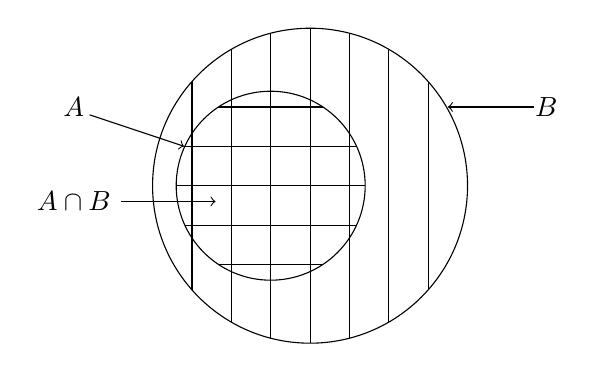
\begin{tikzpicture}
\begin{scope}
\clip[draw] (0,0) circle[radius=1.2];
\foreach \y in {-1.5,-1,-.5,0,.5,1,1.5}
  \draw (-2,\y) -- (2,\y);
\end{scope}
\begin{scope}
\clip[draw] (.5,0) circle[radius=2];
\foreach \x in {-1,-.5,0,.5,1,1.5,2}
  \draw (\x,-2) -- (\x,2);
\end{scope}
\node at (3.5,1) {$B$};
\node at (-2.5,1) {$A$};
\node at (-2.5,-.2) {$A\cap B$};
\draw[->] (3.35,1) -- ++(-1.1,0);
\draw[->] (-2.3,.9) -- ++(1.2,-.4);
\draw[->] (-1.9,-.2) -- ++(1.2,0);
\end{tikzpicture}
\end{center}


\item
אם נתון יחס בין ההסתברות של מאורע וההסתברות של המשלים למאורע אפשר לחשב את ההסתברויות:
\begin{eqn}
P(X)&=&4P(\overline{X})\\
P(X)&=&4(1-P(X))\\
P(X)&=&1/5\,.
\end{eqn}

\end{itemize}
